%%%%%%%%%%%%%%%%%%%%%%%%%%%%%%%%%%%%%%%%%
% Jacobs Landscape Poster
% LaTeX Template
% Version 1.0 (29/03/13)
%
% Created by:
% Computational Physics and Biophysics Group, Jacobs University
% https://teamwork.jacobs-university.de:8443/confluence/display/CoPandBiG/LaTeX+Poster
% 
% Further modified by:
% Nathaniel Johnston (nathaniel@njohnston.ca)
%
% This template has been downloaded from:
% http://www.LaTeXTemplates.com
%
% License:
% CC BY-NC-SA 3.0 (http://creativecommons.org/licenses/by-nc-sa/3.0/)
%
%%%%%%%%%%%%%%%%%%%%%%%%%%%%%%%%%%%%%%%%%

%----------------------------------------------------------------------------------------
%	PACKAGES AND OTHER DOCUMENT CONFIGURATIONS
%----------------------------------------------------------------------------------------

\documentclass[final]{beamer}

\usepackage[scale=1.24]{beamerposter} % Use the beamerposter package for laying out the poster

\usetheme{confposter} % Use the confposter theme supplied with this template

\setbeamercolor{block title}{fg=ngreen,bg=white} % Colors of the block titles
\setbeamercolor{block body}{fg=black,bg=white} % Colors of the body of blocks
\setbeamercolor{block alerted title}{fg=white,bg=dblue!70} % Colors of the highlighted block titles
\setbeamercolor{block alerted body}{fg=black,bg=dblue!10} % Colors of the body of highlighted blocks
% Many more colors are available for use in beamerthemeconfposter.sty

%-----------------------------------------------------------
% Define the column widths and overall poster size
% To set effective sepwid, onecolwid and twocolwid values, first choose how many columns you want and how much separation you want between columns
% In this template, the separation width chosen is 0.024 of the paper width and a 4-column layout
% onecolwid should therefore be (1-(# of columns+1)*sepwid)/# of columns e.g. (1-(4+1)*0.024)/4 = 0.22
% Set twocolwid to be (2*onecolwid)+sepwid = 0.464
% Set threecolwid to be (3*onecolwid)+2*sepwid = 0.708

\newlength{\sepwid}
\newlength{\onecolwid}
\newlength{\onepointfivecolwid}
\newlength{\twocolwid}
\newlength{\threecolwid}
\setlength{\paperwidth}{46.81in} % A0 width: 46.8in
\setlength{\paperheight}{33.11in} % A0 height: 33.1in
\setlength{\sepwid}{0.02\paperwidth} % Separation width (white space) between columns
\setlength{\onecolwid}{0.22\paperwidth} % Width of one column
\setlength{\onepointfivecolwid}{0.33\paperwidth}
\setlength{\twocolwid}{0.464\paperwidth} % Width of two columns
\setlength{\threecolwid}{0.708\paperwidth} % Width of three columns
\setlength{\topmargin}{-0.5in} % Reduce the top margin size
%-----------------------------------------------------------

\usepackage{graphicx}  % Required for including images

\usepackage{booktabs} % Top and bottom rules for tables
\usepackage{multirow}
\usepackage[most]{tcolorbox}

%----------------------------------------------------------------------------------------
%	TITLE SECTION 
%----------------------------------------------------------------------------------------

\title{Towards Neural Machine Translation for Edoid Languages}	

\author{Iroro Fred \d{\`O}n\d{\`o}m\d{\`e} Orife} % Author(s)

\institute[affiliations]{Niger-Volta Language Technologies Institute} % Institution(s)

%----------------------------------------------------------------------------------------

\begin{document}

\addtobeamertemplate{block end}{}{\vspace*{0.5ex}} % White space under blocks
\addtobeamertemplate{block alerted end}{}{\vspace*{0.5ex}} % White space under highlighted (alert) blocks

\setlength{\belowcaptionskip}{0.5ex} % White space under figures
\setlength\belowdisplayshortskip{0.5ex} % White space under equations

\addtobeamertemplate{headline}{} 
{
\begin{tikzpicture}[remember picture,overlay] 
\node [shift={(-22 cm,-10cm)}] at (current page.north east) {\includegraphics[height=3cm]{logos/AI-logo}}; 
\end{tikzpicture} 
}
\addtobeamertemplate{headline}{} 
{
%\begin{tikzpicture}[remember picture,overlay] 
%\node [shift={(-10 cm,-10cm)}] at (current page.north east) {\includegraphics[height=3cm]{logos/fair-wordmark-style-1}}; 
%\end{tikzpicture} 
}
\addtobeamertemplate{headline}{} 
{
%\begin{tikzpicture}[remember picture,overlay] 
%\node [shift={(10 cm,-10cm)}] at (current page.north west) {
%\includegraphics[height=3cm]{logos/nyu_short_color}
%}; 
%\end{tikzpicture} 
}

% Code Link

\addtobeamertemplate{headline}{} 
{
\begin{tikzpicture}[remember picture,overlay] 
\node [shift={(-14 cm,6cm)}] at (current page.south east) {
\begin{tcolorbox}[colback=blue!5!white,colframe=blue!75!black,width=\onecolwid]
  \begin{minipage}{.3\textwidth}
  
\includegraphics[width=\textwidth]{links/qr_code_blue_bg}
  \end{minipage} \quad
  \begin{minipage}{.6\textwidth}
  {\normalsize
  Code (Github) \\
\href{https://github.com/Niger-Volta-LTI/edoid-nmt}{Niger-Volta-LTI/edoid-nmt}
  }
  \end{minipage}
  \end{tcolorbox}
}; 
\end{tikzpicture} 
}

% Paper Link

\addtobeamertemplate{headline}{} 
{
\begin{tikzpicture}[remember picture,overlay] 
\node [shift={(16.5 cm,6cm)}] at (current page.south west) {
  \begin{tcolorbox}[colback=blue!5!white,colframe=blue!75!black,width=\onecolwid]
  \begin{minipage}{.3\textwidth}
  
\includegraphics[width=\textwidth]{links/qr_paper_blue_bg}
  \end{minipage} \quad
  \begin{minipage}{.6\textwidth}
  {\normalsize
    Paper (arXiv) \\
    \href{https://arxiv.org/abs/2003.10704}{2003.10704}
  }
  \end{minipage}
  \end{tcolorbox}
}; 
\end{tikzpicture} 
}

\begin{frame}[t] % The whole poster is enclosed in one beamer frame

\begin{columns}[t] % The whole poster consists of three major columns, the second of which is split into two columns twice - the [t] option aligns each column's content to the top

\begin{column}{\sepwid}\end{column} % Empty spacer column

\begin{column}{\onecolwid} % The first column

%----------------------------------------------------------------------------------------
%	OBJECTIVES
%----------------------------------------------------------------------------------------

\begin{block}{Overview}

Many of the 500 plus languages spoken in Nigeria today have relinquished their previous prestige and purpose in modern society to English and Nigerian Pidgin, notably amongst the younger generations.

\vspace{10mm}

% How language inequality affects people and indigenous language research
For tens of millions of speakers, language inequalities manifest themselves as unequal access to information, communications, health care, security along with attenuated participation in political and civic life \cite{odojelanguage, awobuluyi201626}.

\end{block}

\vspace{5mm}

\begin{block}{}

\vspace{-15mm}

\begin{center}
% \includegraphics[trim=left bottom right top, clip]{file}
 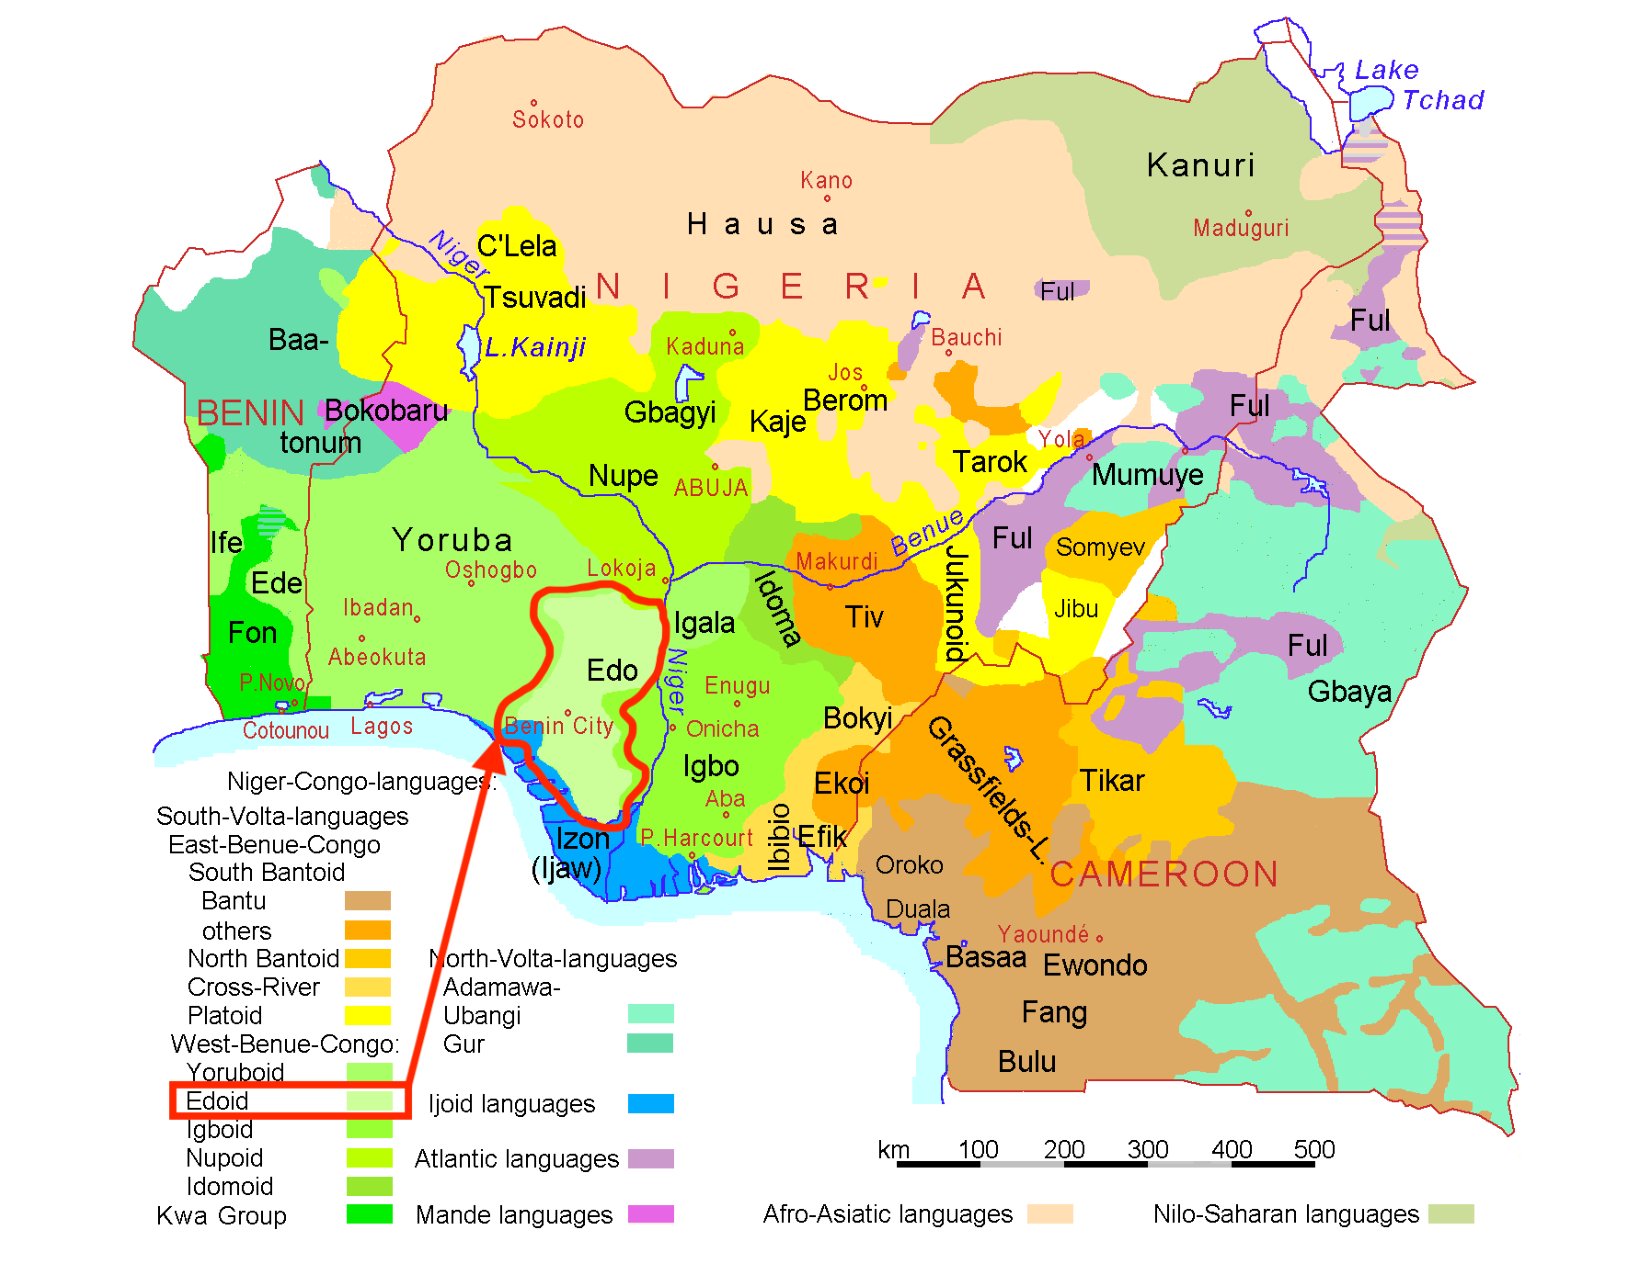
\includegraphics[trim = 25mm 0mm 5mm 3mm, clip, width=1.2\textwidth]{figures/Edoid.pdf}
\end{center}

\vspace{5mm}

Machine Translation (MT) can facilitate good governance, national development and offers a path for technological, economic, social and political participation and empowerment to those with unequal access. 

\end{block}

\vspace{5mm}

\end{column} % End of the first column

\begin{column}{\sepwid}\end{column} % Empty spacer column

\begin{column}{\onecolwid}


\begin{block}{This Work}

Using the new JW300 public dataset, we trained and evaluated baseline Neural Machine Translation (NMT) models for four widely spoken Edoid languages listed below with their classification from \cite{elugbe1989comparative}. \\

\vspace{5mm}

% Population figures: https://en.wikipedia.org/wiki/Edoid_languages
% 
% Edo: Wikipedia ~1.6 million speakers (2015)
% - 1.8M https://joshuaproject.net/people_groups/11714/NI (Ethnologue 2016)
% - https://kwekudee-tripdownmemorylane.blogspot.com/2013/06/edo-people-africas-most-popular-and.html  (percentages)
% - http://www.edostate.gov.ng/edo-people/ (4 Million x 57.54% = 2.3M)

% Esan: 628k https://joshuaproject.net/people_groups/11153/NI (Ethnologue 2016)

% Urhobo: https://en.wikipedia.org/wiki/Urhobo_people
% 2 Million people upperbound?, assuming only a % are native speakers
% 1.2 - 1.5 Million people as of 2004: 
% - http://www.waado.org/urhobo_kinsfolk/archive/Conferences/fifth_annual/academic/urhobo_language_mowarin.html
% 1.068M - https://joshuaproject.net/people_groups/15728/NI (Ethnologue 2016)

% Isoko: https://en.wikipedia.org/wiki/Isoko_language ~500k
% 658k https://joshuaproject.net/people_groups/12266/NI (Ethnologue 2016)


\begin{table}[h]
\begin{center}
\begin{tabular}{cccc}
  \textbf{Language} &  & \textbf{Branch} & \textbf{\# Speakers} \\
  \specialrule{3pt}{2pt}{10pt}
  \d{\`E}d{\'o}  &  & North-Central & \textasciitilde{1.6 - 2.3M} \\
  {\'E}s{\'a}n & & North-Central & \textasciitilde{630k} \\
    \midrule
  Urhobo  & & Southwestern &  \textasciitilde{1 - 1.5M} \\
  Isoko   & & Southwestern & \textasciitilde{660k} \\
  \specialrule{3pt}{2pt}{2pt}
  \end{tabular}
\end{center}
\end{table}


\vspace{15mm}

\textbf{Dataset:}
JW300 dataset is a large-scale, parallel corpus comprising more than 300 languages of which 101 are African. JW300 text is drawn from the Watchtower and Awake! religious magazines by Jehovah's Witnesses (JW). The test set contains sentences with the highest coverage across all other languages in the corpus. \\

\vspace{10mm}

\textbf{Models:} The open-source, Python 3 machine translation toolkit \texttt{JoeyNMT} was used to train Transformer models \cite{NIPS2017_7181}. Our training hardware was the free-tier configuration on Google Colaboratory, a single core Xeon CPU instance and a Tesla K80 GPU.

\end{block}

\begin{block}{Experimental Setup}

  We trained baseline Transformer models for each langauge using:
\begin{description}
  \item[$\bullet$] Byte Pair Encoding (BPE) subword tokenization
  \item[$\bullet$] Word-level tokenization.
\end{description}

For BPE, 4000 BPE tokens were used based on ablation study by Martinus et al. for South African languages \cite{focus_southafrica}.

\end{block}

\end{column} % End of the second column

% % % % 

\begin{column}{\sepwid}\end{column} % Empty spacer column

\begin{column}{\twocolwid} % The third column

\begin{block}{Results}

\begin{center}
Per-language BLEU scores by BPE or word-level tokenization
% \includegraphics[trim=left bottom right top, clip]{file}
  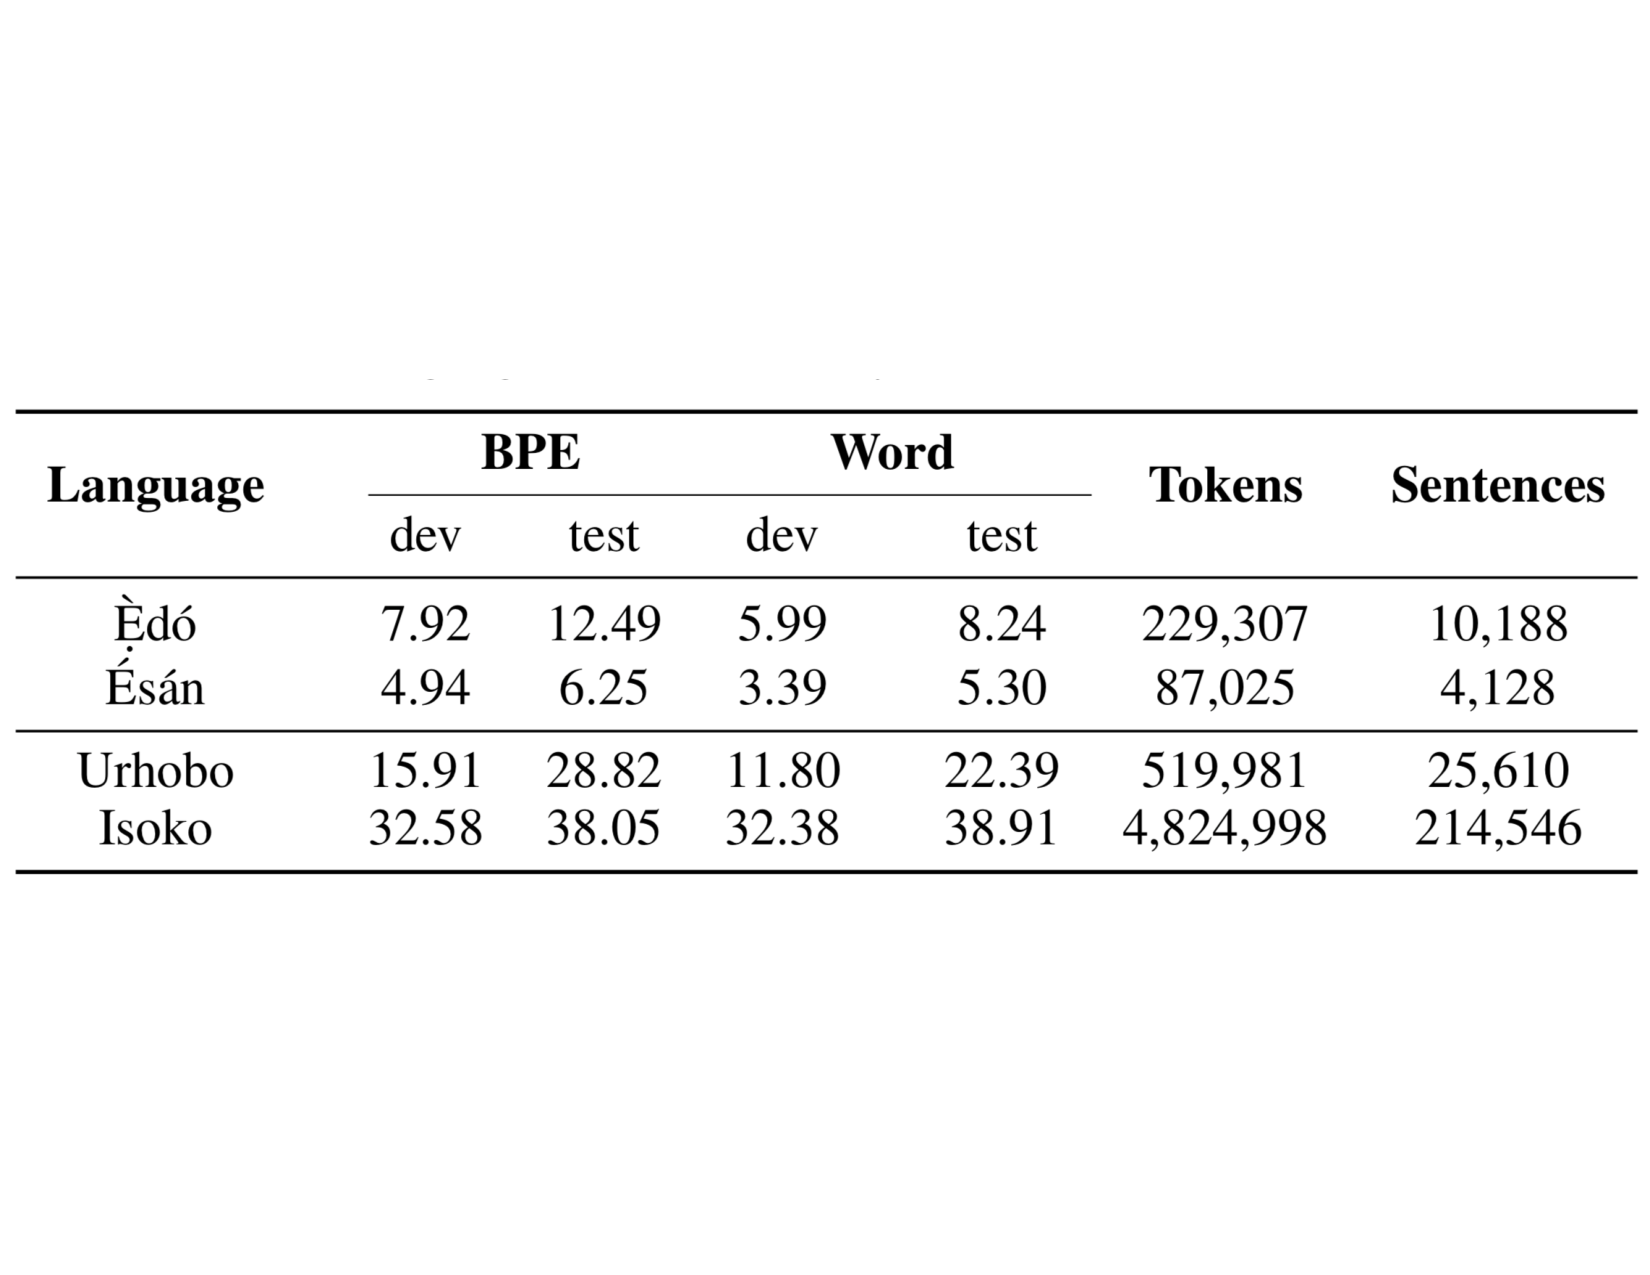
\includegraphics[trim = 0mm 60mm 0mm 55mm, clip, width=0.8\textwidth]{figures/edoid_nmt_results.pdf}
\end{center}

%\begin{table}[h]
%\label{results}
%\begin{center}
%\begin{tabular}{c@{\qquad}ccc@{\qquad}ccc}
%  \specialrule{3pt}{2pt}{13pt}
%  \multirow{2}{*}{\raisebox{-\heavyrulewidth}{\textbf{Language}}} & \multicolumn{2}{c}{\textbf{BPE}} & \multicolumn{2}{c}{\textbf{Word}} & \multirow{2}{*}{\raisebox{-\heavyrulewidth}{\textbf{Tokens}}} & \multirow{2}{*}{\raisebox{-\heavyrulewidth}{\textbf{Sentences}}}
%  	 \\
%  \cmidrule{2-5}
%  & dev & test & dev & test \\
%  \midrule
%  \d{\`E}d{\'o}  & 7.92 & 12.49 & 5.99 & 8.24 &  229,307 & 10,188 \\
%  {\'E}s{\'a}n & 4.94 & 6.25 & 3.39 & 5.30 & 87,025 & 4,128 \\
%    \midrule
%  Urhobo  & 15.91 & 28.82 & 11.80 & 22.39 & 519,981 & 25,610 \\
%  Isoko   & 32.58 & 38.05 & 32.38 & 38.91 & 4,824,998 & 214,546 \\
%  \specialrule{3pt}{2pt}{2pt}
%  \end{tabular}
%\end{center}
%\end{table}

\end{block}

\begin{columns}[t,totalwidth=\twocolwid] % Split up the two columns wide column again

\begin{column}{\onecolwid} % The first column within column 2 (column 2.1)



\begin{block}{Analysis}

\begin{itemize}
\item Urhobo and Isoko translation quality was generally \textbf{satisfactory} when reviewed by L1 speakers, correlating with higher BLEU scores.
\item BPE tokenization provided \textbf{\textasciitilde{37\%} boost} for \d{\`E}d{\'o} and {\'E}s{\'a}n, a \textbf{32\% boost} for Urhobo but was flat to slightly \textbf{worse} than word-level tokenization for Isoko.
\item The performance of the Isoko models, with BLEU scores in the range \{32, 39\}, gives an estimate of how much \textbf{additional clean text} is required to achieve a similar performance with \d{\`E}d{\'o} and {\'E}s{\'a}n.
\item A full ablation study with different (subword) tokenization approaches is needed to discover a more optimal representation.
\item A \textbf{human evaluation study} and extensive error analysis will be crucial to better understand the linguistic features where NMT models under-perform.
\item Future work include investigations using unsupervised machine translation and back-translation.
\end{itemize}

\end{block}

%----------------------------------------------------------------------------------------

\end{column} % End of column 2.1

\begin{column}{\onecolwid} % The second column within column 2 (column 2.2)

\begin{block}{References}

% {\small
% [Lazaridou et al., 2016] Lazaridou, Angeliki and Peysakhovich, Alexander and Baroni, Marco (2016). \\
% Multi-agent cooperation and the emergence of (natural) language. \\
% \href{https://arxiv.org/abs/1612.07182}{In Proceedings of ICLR}

% \vspace{5mm}

% [Jorge et al., 2016] Jorge, Emilio and K{\aa}geb{\"a}ck, Mikael and Gustavsson, Emil (2016). \\
% Learning to Play Guess Who? and Inventing a Grounded Language as a Consequence. \\
% \href{https://arxiv.org/abs/1611.03218}{arXiv preprint arXiv:1611.03218}
% }

\nocite{*} % Insert publications even if they are not cited in the poster
\footnotesize{\bibliographystyle{apalike}
\bibliography{main}\vspace{0.75in}}

\end{block}

\end{column} % End of column 2.2

\end{columns} % End of the split of column 2



\end{column} % End of the third column

\end{columns} % End of all the columns in the poster

\end{frame} % End of the enclosing frame

\end{document}
